\chapter{Dasar Teori}
\label{chap: dasarTeori}
		
\section{CodeIgniter}
\label{sec: codeigniter}

	CodeIgniter merupakan sebuah peralatan bagi orang-orang yang ingin membuat sebuah \textit{web} dengan menggunakan bahasa PHP. CodeIgniter sendiri dibuat dengan tujuan memungkinkan pengembangan proyek-proyek lebih cepat daripada menuliskan kode dari awal. Tujuan tersebut di wujudkan dengan tersedianya \textit{library} yang berisi \textit{task} yang biasa dibutuhkan dalam pengembangan program dibarengi dengan antarmuka yang sederhana serta struktur logika untuk mengakses \textit{library} tersebut. Dengan begitu dapat disimpulkan bahwa CodeIgniter membuat pemrogram fokus pada kreativitas pembuatan program dengan meminimalkan jumlah kode yang dituliskan.
	
	\subsection{Flowchart Aplikasi CodeIgniter}
	\label{sub: FlowAppCI}
	
	Pada gambar \ref{fig:flowchartCI} menunjukkan \textit{flowchart} aliran data pada CodeIgniter:
	\begin{figure}[H]
		\centering
		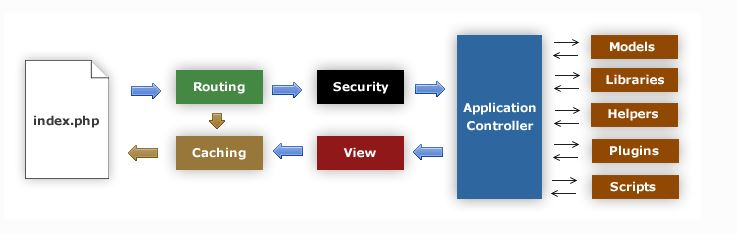
\includegraphics[scale=0.75]{Gambar/flowChartCI}
		\caption{Flowchart CodeIgniter}
		\label{fig:flowchartCI}
	\end{figure}
	
	Keterangan:
	\begin{enumerate}
		\item Index.php berfungsi sebagai pengontrol utama, yang menginisialisasikan sumber-sumber yang diperlukan untuk menjalankan CodeIgniter.
		\item \textit{Router} akan memeriksa permintaan HTTP untuk menentukan apa yang harus dilakukan selanjutnya
		\item Jika terdapat \textit{cache}, maka cache tersebut akan dikirim langsung ke browser dengan menjalankan sistem eksekusi normal.
		\item  HTTP \textit{request} dan data yang diserahkan oleh \textit{user} akan disaring oleh sistem keamanan terlebih dahulu oleh bagian keamanan(\textit{security}) dari CodeIgniter yang dijalankan sebelum \textit{controller} dari aplikasi diisi.
		\item \textit{Application Controller} akan mengambil isi dari \textit{model, libraries, helpers, plugins, scripts}, dan sumber lain yang diperlukan untuk menjalankan perintah-perintah spesifik.
		\item Kemudian \textit{View} akan diterjemahkan dari \textit{Application Controller} dan dikirim ke \textit{web browser} untuk kemudian ditampilkan. Jika pada view final terdapat \textit{file cache}, maka view tersebut akan terlebih dahulu dilakukan \textit{cached} sehingga permintaan berikutnya dapat dilayani.
	\end{enumerate}
	
	\subsection{Model-View-Controller}
	\label{sub: MVC}
	
	CodeIgniter menggunakan dasar pola pengembangan \textit{Model-View-Controller}(MVC). Pola pengembangan MVC ini merupakan suatu pendekatan yang memisahkan antara pengerjaan logika dan tampilan dari aplikasi.
	
	MVC sendiri terdiri dari 3 bagian, yaitu:
	\begin{enumerate}
		\item \textit{Model} merepresentasikan struktur data. Secara khusus, \textit{model} merupakan kelas yang membantu menangani kueri-kueri sql seperti \textit{insert, update,}dan \textit{delete} pada basis data.
		\item \textit{View} merepresentasikan informasi yang ditunjukkan kepada pengguna. Sebuah \textit{view} biasanya berbentuk \textit{web page}, tetapi dalam CodeIgniter \textit{view} bisa berbentuk \textit{header, footer,} dan berbagai jenis \textit{page} lainnya.
		\item \textit{Controller} berfungsi sebagai perantara antara \textit{Model}, \textit{View}, dan sumber daya lain yang diperlukan untuk memproses HTTP \textit{request} dan menghasilkan halaman web.
	\end{enumerate}
	

	
\section{AngularJS}
\label{sec: angularJS}
	
	AngularJS merupakan sebuah \textit{framework} terstruktur yang digunakan untuk aplikasi web yang bersifat dinamis. Hal tersebut memungkinkan \textit{programmer} untuk mempergunakan HTML sebagai template bahasa pemrograman dan memperluas sintaks HTML agar dapat mengekspresikan komponen aplikasi dengan jelas dan ringkas. Sifat AngularJS yang mengikat data dan mempunyai ketergantungan injeksi akan menghilangkan banyak kode yang seharusnya dituliskan oleh \textit{programmer}, dan semua itu terjadi pada \textit{browser} sehingga dapat disimpulkan bahwa AngularJS merupakan pasangan yang sangat ideal bagi penggunaan teknologi server. 
	Dalam pembuatannya, ketidakcocokkan halaman statik dan dinamik biasanya diselesaikan dengan pendekatan sebagai berikut:
	\begin{enumerate}
		\item \textit{Library}: merupakan sebuah koleksi dari berbagai macam fungsi yang berguna dalam pembuatan aplikasi \textit{web}, contoh: JQuery.
		\item \textit{Frameworks}: merupakan suatu implementasi dari sebuah aplikasi \textit{web} yang menempatkan kode yang dituliskan secara detail. \textit{Framework} akan berperan melakukan pemanggilan ke kode yang dituliskan \textit{programmer} ketika aplikasi membutuhkan sesuatu yang spesifik, contoh: durandal, ember, dll.
	\end{enumerate}
	
	Dalam pembentukannya, AngularJS memiliki pendekatan yang berbeda. AngularJS berupaya untuk meminimalkan ketidakcocokan antara dokumen utama dari HTML dengan apa yang dibutuhkan oleh aplikasi untuk membuat konstruksi HTML baru. AngularJS mengajarkan \textit{browser} sintaks baru yang disebut \textit{directives}. Contoh contoh \textit{directives} adalah:
	\begin{enumerate}
		\item Keterikatan data di dalam \{\{\}\};
		\item Dukungan untuk \textit{Form} dan \textit{Form Validation}
		\item Pengelompokkan HTMl menjadi komponen - komponen yang dapat dipakai kembali.
	\end{enumerate}
	
	\subsection{Gambaran Konseptual}
	\label{sub: gambaranKonsep}
		Berikut ini adalah beberapa bagian-bagian terpenting dalam AngularJS.
		\begin{center}
			\begin{tabular}{| m{5cm} | m{10cm} |}
				\hline
				Konsep & Deskripsi \\
				\hline
				Template & HTML dengan tambahan markup \\
				\hline
				Directives & Pengembangan HTML dengan atribut dan elemen yang dibuat khusus \\
				\hline
				Model & Data yang ditunjukan kepada pengguna pada tampilan dan bagaimana penguna berinteraksi \\
				\hline
				Scope & Konteks dimana model disimpan, sehingga controller, directives dan expression dapat mengaksesnya \\
				\hline
				Expression & Mengakses variabel dan fungsi dari scope \\
				\hline
				Compiler & Menguraikan template, directives, dan expression \\
				\hline
				Filter & Mengatur nilai dari sebuah expression untuk di tunjukkan kepada pengguna \\
				\hline
				View & Apa yang akan dilihat oleh pengguna (DOM) \\
				\hline
				Data Binding & Menyelaraskan data yang ada pada \textit{model} dan view \\
				\hline
				Controller & Mengatur logika dibalik tampilan \\
				Dependency Injection & Membuat dan menyambungkan objek dan fungsi \\
				\hline
				Injector & Tempat penyimpanan dependency Injection \\
				\hline
				Module & Tempat penyimpanan untuk bagian-bagian yang berbeda dalam sebuah aplikasi, yang mencakup: controllers, services, filters, directives yang mengkonfigurasika injector \\
				\hline
				Services & Logika bisnis independen dari views yang bisa dipakai kembali  \\
				\hline
				\end{tabular}
			\end{center}
	
	\subsection{Data Binding}
	\label{sub: dataBinding}
		
		\textit{Data Binding} pada AngularJS merupakan penyelarasan data antara \textit{model} dan komponen - komponen \textit{view}. Ketika \textit{model} berubah, maka \textit{view} pun akan berubah, begitu juga dengan sebaliknya.
		
		\begin{figure}[H]
			\centering
			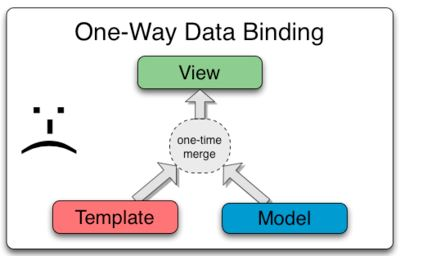
\includegraphics[scale=0.75]{Gambar/Dabin1}
			\caption{Data Binding Classical Templates System}
			\label{fig:dabin1}
		\end{figure}
		Pada gambar \ref{fig:dabin1} menjelaskan bahwa kebanyakan \textit{data binding} adalah proses satu arah. Hal itu dilakukan dengan menyatukan \textit{template} dan \textit{model} menjadi \textit{view}. Setelah penyatuan, pergantian pada \textit{model} tidak secara otomatis mengganti \textit{view} yang sudah ditampilkan.
		\begin{figure}[H]
			\centering
			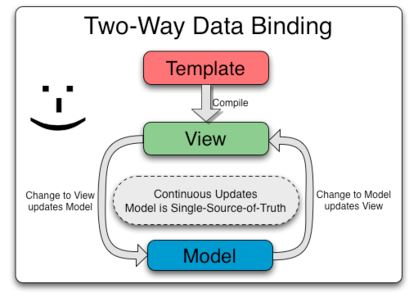
\includegraphics[scale=0.75]{Gambar/Dabin2}
			\caption{Data Binding pada Angular}
			\label{fig:dabin2}
		\end{figure}
		Pada gambar \ref{fig:dabin2} menjelaskan perbedaan yang diberikan oleh pelaksanaan \textit{data binding} pada AngularJS. Pertama, \textit{template} akan di \textit{compile} pada browser. Hasil dari \textit{compile} tersebut adalah \textit{live view}. Pada tahap ini perubahan yang terjadi di \textit{view} akan disampaikan kepada \textit{model}, dan perubahan yang terjadi pada \textit{model} akan mengubah \textit{view}.
		
		Karena \textit{view} merupakan proyeksi dari \textit{model}, menyebabkan \textit{controller} benar-benar terpisahkan dari \textit{view} tanpa disadari. Hal ini mempermudah pengujian \textit{controller}, karena terisolasi tanpa adanya \textit{view} dan DOM( \textit{browser dependency}).
		
\section{Twitter Bootstrap}
\label{sec: Bootrstrap}

		